\quad Testovi su izvođeni na već opisanoj verziji igre \textit{2048}. Verzija se ispostavila problematičnom jer je brzina izvođenja igre bitno ograničena implementacijom verzije. U svim testovima svi su programi imali tri pokušaja rješavanja igre. U slučaju veličine populacije četiri, prosječno vrijeme potrebno za prolazak svih programa generacije kroz igru bilo je petnaest minuta. U slučaju veličine populacije osam, prosječno vrijeme prolaska generacije kroz igru bilo je trideset minuta. U slučaju veličine populacije šesnaest, prosječno vrijeme prolaska generacije kroz igru bilo je šezdeset minuta. Povećanje potrebnog vremena je linearne zavisnosti i učinilo je treniranje predugim za ikakve prave rezultate. Rezultati koji su prikupljeni za različite arhitekture i parametre sustava ograničeni su na tridesetu generaciju kako bi se mogli međusobno usporediti. Ograničenje je takvo zbog toga što je to minimalna generacija do koje su došli svi testovi prije zaustavljanja daljnjeg treniranja. 
\par
Provedeno je pet testova s četiri različite arhitekture i s različitim parametrima sustava. Radi jednostavnosti zapisa ispod slika uvodimo kratice: c - broj stupaca, r - broj redova, p - veličina populacije, f - broj funkcija, m - broj mutacija po djetetu.
 \par
 Prvi test izveden je nad arhitekturom mreže sa širinom šesnaest i dubinom četiri uz veličinu populacije četiri, broj funkcija četiri (+,-,*,/) i jednom single mutacijom po djetetu. Selekcija se provodi nad četiri programa. Korišteno je križanje koje je prvo opisano u potpoglavlju 8.5. Test je osmišljen kao reprezentacija općenite i plitke mreže sa širinom većom od nula, a u ovom slučaju širina je jednaka broju ulaza. Trajanje testiranja bilo je 24 sata, unutar kojih je sustav prošao kroz sedamdeset i dvije generacije. Većina rezultata nalazila se u rasponu 70-150. Na slici 9.1 možemo vidjeti najbolje srednje vrijednosti rezultata od nulte do tridesete generacije. Iako oscilacije postoje, vidimo polagani rast najboljih rezultata do petnaeste generacije gdje započinje stagnacija i lagan pad. Na osnovu rezultata daljnjih generacija, srednje vrijednosti rezultata stagniraju ili se nalaze unutar istog raspona rezultata.
 \begin{figure}[h]
 	\centering
 	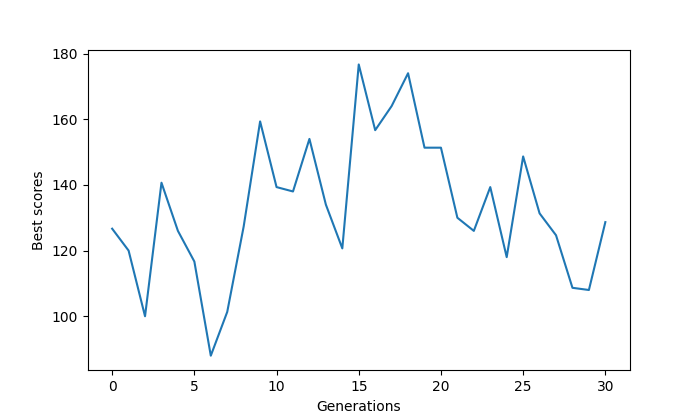
\includegraphics[width=0.9\linewidth]{graph_1}
 	\caption{Najbolje srednje vrijednosti rezultata programa za c=4, r=16, p=4, f=4, m=1}
 \end{figure}\newpage
\par
Drugi test izveden je nad arhitekturom mreže sa širinom jedan i dubinom sto uz veličinu populacije četiri, broj funkcija četiri (+,-,*,/) i jednom single mutacijom po djetetu. Selekcija je provedena nad četiri programa. Korišteno je križanje s jednom točkom prijeloma. Test je osmišljen kao reprezentacija jednostavnog slučaja mreže širine jedan gdje je naglasak na vezama između čvorova u dubini. Ideja je bila koristiti ovaj slučaj kao bazu za uspoređivanje s drugim arhitekturama i parametrima sustava. Trajanje testiranja bilo je 22 sata, unutar koji je sustav prošao kroz pedeset i tri generacije. Većina rezultata nalazila se u rasponu 90-150. Na slici 9.2 možemo vidjeti najbolje srednje vrijednosti rezultata od nulte do tridesete generacije. Primjećuje se porast najbolje srednje vrijednosti do dvadeset i treće generacije nakon čega slijedi nagli pad uspješnosti i povratak u stanje prije pada. Rezultati daljnjih generacija ukazuju na umjereno poboljšanje, ali gornja granica raspona većine rezultata ne pomiče se previše.
\par 
Treći test je gotovo po svim parametrima jednak prošlom. Jedina razlika je veličina populacije. U ovom testu veličina populacije je 8. Cilj ovog testa bio je vidjeti razliku u uspješnosti kroz generacije ako povećamo veličinu populacije. Trajanje testiranja bilo je 20 sati, unutar kojih je sustav prošao kroz trideset i dvije generacije. Većina rezultata nalazi se u rasponu od 80-150. Počinjemo uviđati iste raspone rezultata kroz testove i sumnja se kako je ovo početni raspon rezultata većine inicijaliziranih populacija. Slika 9.3 prikazuje najveće srednje vrijednosti rezultata od nulte do tridesete generacije. Stabilan porast rezultata u ovom testu kasni za onim u prošlom testu. Minimalna i maksimalna vrijednost rezultata je veća od prošlog testa, iako je razlika možda zanemariva.

 \begin{figure}[h]
	\centering
	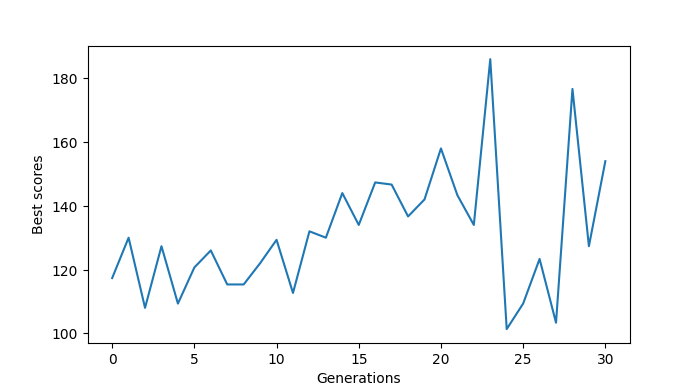
\includegraphics[width=0.9\linewidth]{graph_2}
	\caption{Najbolje srednje vrijednosti rezultata programa za c=100, r=1, p=4, f=4, m=1}
\end{figure}

 \begin{figure}[h]
	\centering
	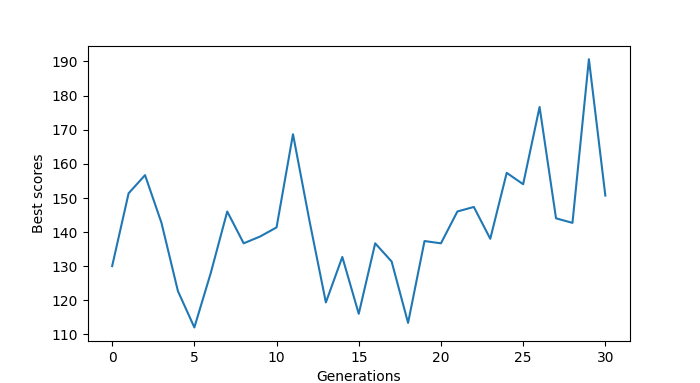
\includegraphics[width=0.9\linewidth]{graph_3}
	\caption{Najbolje srednje vrijednosti rezultata programa za c=100, r=1, p=8, f=4, m=1}
\end{figure}

\par
U četvrtom testu dubina je povećana na dvjesto i uvedene su još dvije funkcije (min i max). Testom se pokušao vidjeti utjecaj produbljavanja mreže i dodavanja dodatnih mogućih funkcija. Trajanje testiranja bilo je 20 sati, unutar kojih je sustav prošao kroz trideset i pet generacija. U početnim generacijama većina rezultata nalazi se u rasponu 100-150, ali u kasnijim generacijama raspon pada na 90-120. Slika 9.4 prikazuje najveće srednje vrijednosti rezultata od nulte do tridesete generacije. Iznos najveće srednje vrijednosti rezultata u generaciji je nestabilan te na odsječku od trideset generacija ne možemo zaključiti previše. Prosjek rezultata po generacijama pokazuje stabilizaciju rezultata, ali i njihov pad. 
 \begin{figure}[h]
	\centering
	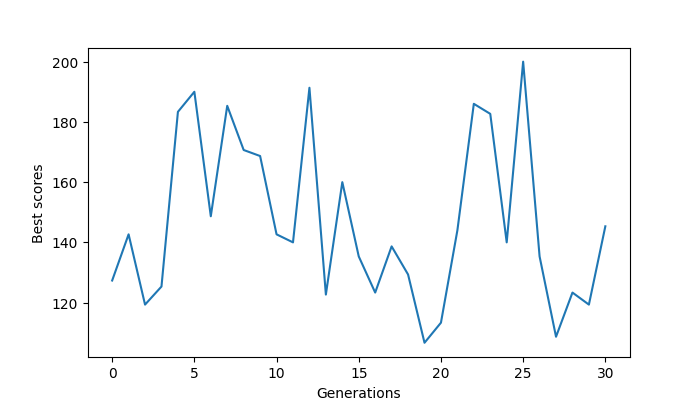
\includegraphics[width=0.9\linewidth]{graph_4}
	\caption{Najbolje srednje vrijednosti rezultata programa za c=200, r=1, p=8, f=6, m=1}
\end{figure}

\par
Peti test nadograđuje četvrti tako da smo mrežu produbili s dodatnih sto čvorova, veličinu populacije postavili na šesnaest, selekcija je provedena nad osam programa i broj single mutacija po djetetu povećali na dva. Cilj testa bio je vidjeti kako će povećanje kompleksnosti i promjenjivosti populacije utjecati na rezultate. Trajanje testiranja bilo je 43 sata, unutar kojih je sustav prošao kroz četrdeset i jednu generaciju. Većina rezultata nalazi se u rasponu od 90-150. Slika 9.5 prikazuje najveće srednje vrijednosti rezultata od nulte do tridesete generacije. Najveća srednja vrijednost rezultata generacije u ovom testu postiže najveći iznos u usporedbi s ostalim testovima. Na žalost ovaj test jedini pokazuje jasan pad najveće srednje vrijednosti rezultata i izrazito je nestabilan s naglim usponima i padovima.  
 \begin{figure}[t]
	\centering
	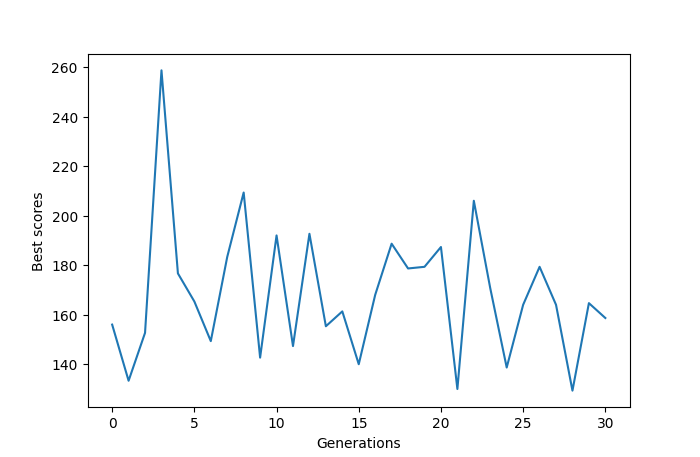
\includegraphics[width=0.9\linewidth]{graph_5}
	\caption{Najbolje srednje vrijednosti rezultata programa za c=300, r=1, p=16, f=6, m=2}
\end{figure}
\par 
Pregledom rezultata testova možemo pretpostaviti nekoliko učinaka koje parametri mogu imati na uspješnost programa. Veća kompleksnost može dovesti do većeg uspjeha programa, ali dovodi i do veće nestabilnosti. Prevelika razina mutacije utječe destruktivno na generacije programa. Povećavanjem populacije, bez povećanja selekcije, može dovesti do odgađanja promjene u populaciji. Sve ove pretpostavke nisu dokazane već su postavljene na osnovu dobivenih rezultata i trebaju se tretirati kao moguće hipoteze za budući rad.
\newpage
\verb| |